%% VIth_SPHERIC_paper_tempalte.tex
%% V1.0
%% 2003/03/20
%% by Benedict Rogers
%% courtesy of nicolas.grenier@ec-nantes
%% courtesy of pierre.maruzewski@epfl.ch
%%
%% NOTE: This text file uses MS Windows line feed conventions. When (human)
%% reading this file on other platforms, you may have to use a text
%% editor that can handle lines terminated by the MS Windows line feed
%% characters (0x0D 0x0A).

% Note that the a4paper option is mainly intended so that authors in
% countries using A4 can easily print to A4 and see how their papers will
% look in print. Authors are encouraged to use U.S.
%
% Also note that the "draftcls" or "draftclsnofoot", not "draft", option
% should be used if it is desired that the figures are to be displayed in
% draft mode.
%
% This paper can be formatted using the peerreviewca
% (instead of conference) mode.
\documentclass[a4paper,conference]{IEEEtran}
% If the IEEEtran.cls has not been installed into the LaTeX system files,
% manually specify the path to it:
% \documentclass[conference]{../sty/IEEEtran}

% Dimensions of margins (DO NOT MODIFY THEM)
\setlength{\textheight}    {23.4cm}%
\setlength{\topmargin}     {-0.8cm}%
\setlength{\headheight}    {0.6cm}%
\setlength{\headsep}       {0.9cm}%

% some very useful LaTeX packages include:

\usepackage{cite}      % Written by Donald Arseneau
                        % V1.6 and later of IEEEtran pre-defines the format
                        % of the cite.sty package \cite{} output to follow
                        % that of IEEE. Loading the cite package will
                        % result in citation numbers being automatically
                        % sorted and properly "ranged". i.e.,
                        % [1], [9], [2], [7], [5], [6]
                        % (without using cite.sty)
                        % will become:
                        % [1], [2], [5]--[7], [9] (using cite.sty)
                        % cite.sty's \cite will automatically add leading
                        % space, if needed. Use cite.sty's noadjust option
                        % (cite.sty V3.8 and later) if you want to turn this
                        % off. cite.sty is already installed on most LaTeX
                        % systems. The latest version can be obtained at:
                        % http://www.ctan.org/tex-archive/macros/latex/contrib/supported/cite/

\usepackage{graphicx}  % Written by David Carlisle and Sebastian Rahtz
                        % Required if you want graphics, photos, etc.
                        % graphicx.sty is already installed on most LaTeX
                        % systems. The latest version and documentation can
                        % be obtained at:
                        % http://www.ctan.org/tex-archive/macros/latex/required/graphics/
                        % Another good source of documentation is "Using
                        % Imported Graphics in LaTeX2e" by Keith Reckdahl
                        % which can be found as esplatex.ps and epslatex.pdf
                        % at: http://www.ctan.org/tex-archive/info/
% NOTE: for dual use with latex and pdflatex, instead load graphicx like:
%\ifx\pdfoutput\undefined
%\usepackage{graphicx}
%\else
%\usepackage[pdftex]{graphicx}
%\fi

% However, be warned that pdflatex will require graphics to be in PDF
% (not EPS) format and will preclude the use of PostScript based LaTeX
% packages such as psfrag.sty and pstricks.sty. IEEE conferences typically
% allow PDF graphics (and hence pdfLaTeX). However, IEEE journals do not
% (yet) allow image formats other than EPS or TIFF. Therefore, authors of
% journal papers should use traditional LaTeX with EPS graphics.
%
% The path(s) to the graphics files can also be declared: e.g.,
% \graphicspath{{../eps/}{../ps/}}
% if the graphics files are not located in the same directory as the
% .tex file. This can be done in each branch of the conditional above
% (after graphicx is loaded) to handle the EPS and PDF cases separately.
% In this way, full path information will not have to be specified in
% each \includegraphics command.
%
% Note that, when switching from latex to pdflatex and vice-versa, the new
% compiler will have to be run twice to clear some warnings.

\usepackage{wasysym}
%\usepackage{psfrag}    % Written by Craig Barratt, Michael C. Grant,
                        % and David Carlisle
                        % This package allows you to substitute LaTeX
                        % commands for text in imported EPS graphic files.
                        % In this way, LaTeX symbols can be placed into
                        % graphics that have been generated by other
                        % applications. You must use latex->dvips->ps2pdf
                        % workflow (not direct pdf output from pdflatex) if
                        % you wish to use this capability because it works
                        % via some PostScript tricks. Alternatively, the
                        % graphics could be processed as separate files via
                        % psfrag and dvips, then converted to PDF for
                        % inclusion in the main file which uses pdflatex.
                        % Docs are in "The PSfrag System" by Michael C. Grant
                        % and David Carlisle. There is also some information
                        % about using psfrag in "Using Imported Graphics in
                        % LaTeX2e" by Keith Reckdahl which documents the
                        % graphicx package (see above). The psfrag package
                        % and documentation can be obtained at:
                        % http://www.ctan.org/tex-archive/macros/latex/contrib/supported/psfrag/

%\usepackage{subfigure} % Written by Steven Douglas Cochran
                        % This package makes it easy to put subfigures
                        % in your figures. i.e., "figure 1a and 1b"
                        % Docs are in "Using Imported Graphics in LaTeX2e"
                        % by Keith Reckdahl which also documents the graphicx
                        % package (see above). subfigure.sty is already
                        % installed on most LaTeX systems. The latest version
                        % and documentation can be obtained at:
                        % http://www.ctan.org/tex-archive/macros/latex/contrib/supported/subfigure/

%\usepackage{url}       % Written by Donald Arseneau
                        % Provides better support for handling and breaking
                        % URLs. url.sty is already installed on most LaTeX
                        % systems. The latest version can be obtained at:
                        % http://www.ctan.org/tex-archive/macros/latex/contrib/other/misc/
                        % Read the url.sty source comments for usage information.

%\usepackage{stfloats}  % Written by Sigitas Tolusis
                        % Gives LaTeX2e the ability to do double column
                        % floats at the bottom of the page as well as the top.
                        % (e.g., "\begin{figure*}[!b]" is not normally
                        % possible in LaTeX2e). This is an invasive package
                        % which rewrites many portions of the LaTeX2e output
                        % routines. It may not work with other packages that
                        % modify the LaTeX2e output routine and/or with other
                        % versions of LaTeX. The latest version and
                        % documentation can be obtained at:
                        % http://www.ctan.org/tex-archive/macros/latex/contrib/supported/sttools/
                        % Documentation is contained in the stfloats.sty
                        % comments as well as in the presfull.pdf file.
                        % Do not use the stfloats baselinefloat ability as
                        % IEEE does not allow \baselineskip to stretch.
                        % Authors submitting work to the IEEE should note
                        % that IEEE rarely uses double column equations and
                        % that authors should try to avoid such use.
                        % Do not be tempted to use the cuted.sty or
                        % midfloat.sty package (by the same author) as IEEE
                        % does not format its papers in such ways.

\usepackage{amsmath}   % From the American Mathematical Society
                        % A popular package that provides many helpful commands
                        % for dealing with mathematics. Note that the AMSmath
                        % package sets \interdisplaylinepenalty to 10000 thus
                        % preventing page breaks from occurring within multiline
                        % equations. Use:
%\interdisplaylinepenalty=2500
                        % after loading amsmath to restore such page breaks
                        % as IEEEtran.cls normally does. amsmath.sty is already
                        % installed on most LaTeX systems. The latest version
                        % and documentation can be obtained at:
                        % http://www.ctan.org/tex-archive/macros/latex/required/amslatex/math/



% Other popular packages for formatting tables and equations include:

%\usepackage{array}
% Frank Mittelbach's and David Carlisle's array.sty which improves the
% LaTeX2e array and tabular environments to provide better appearances and
% additional user controls. array.sty is already installed on most systems.
% The latest version and documentation can be obtained at:
% http://www.ctan.org/tex-archive/macros/latex/required/tools/

% Mark Wooding's extremely powerful MDW tools, especially mdwmath.sty and
% mdwtab.sty which are used to format equations and tables, respectively.
% The MDWtools set is already installed on most LaTeX systems. The lastest
% version and documentation is available at:
% http://www.ctan.org/tex-archive/macros/latex/contrib/supported/mdwtools/


% V1.6 of IEEEtran contains the IEEEeqnarray family of commands that can
% be used to generate multiline equations as well as matrices, tables, etc.


% Also of notable interest:

% Scott Pakin's eqparbox package for creating (automatically sized) equal
% width boxes. Available:
% http://www.ctan.org/tex-archive/macros/latex/contrib/supported/eqparbox/



% Notes on hyperref:
% IEEEtran.cls attempts to be compliant with the hyperref package, written
% by Heiko Oberdiek and Sebastian Rahtz, which provides hyperlinks within
% a document as well as an index for PDF files (produced via pdflatex).
% However, it is a tad difficult to properly interface LaTeX classes and
% packages with this (necessarily) complex and invasive package. It is
% recommended that hyperref not be used for work that is to be submitted
% to the IEEE. Users who wish to use hyperref *must* ensure that their
% hyperref version is 6.72u or later *and* IEEEtran.cls is version 1.6b
% or later. The latest version of hyperref can be obtained at:
%
% http://www.ctan.org/tex-archive/macros/latex/contrib/supported/hyperref/
%
% Also, be aware that cite.sty (as of version 3.9, 11/2001) and hyperref.sty
% (as of version 6.72t, 2002/07/25) do not work optimally together.
% To mediate the differences between these two packages, IEEEtran.cls, as
% of v1.6b, predefines a command that fools hyperref into thinking that
% the natbib package is being used - causing it not to modify the existing
% citation commands, and allowing cite.sty to operate as normal. However,
% as a result, citation numbers will not be hyperlinked. Another side effect
% of this approach is that the natbib.sty package will not properly load
% under IEEEtran.cls. However, current versions of natbib are not capable
% of compressing and sorting citation numbers in IEEE's style - so this
% should not be an issue. If, for some strange reason, the user wants to
% load natbib.sty under IEEEtran.cls, the following code must be placed
% before natbib.sty can be loaded:
%
% \makeatletter
% \let\NAT@parse\undefined
% \makeatother
%
% Hyperref should be loaded differently depending on whether pdflatex
% or traditional latex is being used:
%
%\ifx\pdfoutput\undefined
%\usepackage[hypertex]{hyperref}
%\else
%\usepackage[pdftex,hypertexnames=false]{hyperref}
%\fi
%
% Pdflatex produces superior hyperref results and is the recommended
% compiler for such use.



% *** Do not adjust lengths that control margins, column widths, etc. ***
% *** Do not use packages that alter fonts (such as pslatex).         ***
% There should be no need to do such things with IEEEtran.cls V1.6 and later.


% correct bad hyphenation here
\hyphenation{op-tical net-works semi-conduc-tor IEEEtran}



\usepackage{fancyheadings}
\usepackage{float}
\usepackage{afterpage}
\usepackage{subfig}
\pagestyle{fancy}

\lhead{$9^{th}$ international SPHERIC workshop}
\rhead{Paris, France, June, 03-05 2014}
\cfoot{} % to avoid page numbering

\newcommand{\OF}{OpenFOAM\textsuperscript{\textregistered}}
\newcommand{\FF}{Fluent\textsuperscript{\textregistered}}
\newcommand{\tauB}{\underline{\underline{\boldsymbol{\tau}}}}
\newcommand{\vv}{\mathbf{v}}
\newcommand{\xx}{\mathbf{x}}
\newcommand{\aaa}{\mathbf{a}}
\newcommand{\ww}{\mathbf{w}}
\newcommand{\gb}{\mathbf{g}}
\newcommand{\nn}{\mathbf{n}}
\newcommand{\yy}{\mathbf{y}}
\newcommand{\Mat}{Matlab{\small$^{\textregistered}$}}


\begin{document}

% paper title
\title{Applications and improvements of the particle finite element method to free surface flows.}


% author names and affiliations
% use a multiple column layout for up to three different
% affiliations
\author{\IEEEauthorblockN{Juan M. Gimenez}
\IEEEauthorblockA{CIMEC\\
Universidad Nacional del Litoral (UNL)\\
Santa Fe, Argentina\\
jmarcelogimenez@gmail.com}
\and
\IEEEauthorblockN{Leo M. Gonz\'{a}lez}
\IEEEauthorblockA{ETSIN\\
Universidad Polit\'{e}cnica de Madrid (UPM)\\
Madrid, Spain\\
leo.gonzalez@upm.es}
\and
\IEEEauthorblockN{Pedro Gal\'{a}n del Sastre}
\IEEEauthorblockA{ETSAM\\
Universidad Polit\'{e}cnica de Madrid (UPM)\\
Madrid, Spain\\
pedro.galan@upm.es}}

% use only for invited papers
%\specialpapernotice{(Invited Paper)}

% make the title area
\maketitle

\begin{abstract}
In this work a new generation of the particle method known as Particle Finite Element Method (PFEM), which combines convective particle movement and fixed mesh resolution, is applied to free surface flows. This methodology, named PFEM-2, presents basically two novel steps: first, the possibility of using larger time steps compared to other similar numerical tools, showing that shorter computational times can be achieved while the solution accuracy is maintained. Second, different improved versions of discontinuous and continuous enriched basis functions for the pressure field have been also developed in order to reconstruct the free surface without artificial diffusion or undesired numerical effects. Combining these two improvements, a variety of free surface flows have been solved in 2D and 3D cases, where the evident advantages of the improvements are remarked.
The results of the different free-surface problems solved which include: Rayleigh-Taylor instability, sloshing problems, viscous standing waves and the dam break problem are compared to well validated numerical alternatives and experimental measurements obtaining good approximations for such complex flows.
\end{abstract}




\section{Introduction}

Hybrid methods are everyday more present in computational fluid mechanics, where the Lagrangian framework given by a particle method is combined with a Eulerian methodology. In these hybrid methods, a fixed or reconstructed every k time steps grid support part of the pressure and velocity calculation. The original idea, given by Monaghan \cite{Mon77} or later works applied to fluid mechanics \cite{Monaghan88} where a pure Lagrangian perspective was used during the whole meshless computation, has been in some cases completed using other well known discretization methods as FVM\cite{Nestor20091733} or FEM\cite{Ide03}. The first combination of Lagrangian methods and FEM methods, known as MFEM \cite{Ide03b}, where a extended Delaunay Tesellation is used to reconstruct the mesh while the fluid evolves. 

The next step in this evolution was the first version of the PFEM method\cite{Idelsohn04}, which was a robust method designed to solve fluid-structure interaction problems including free-surface, breaking waves, flow separations, etc... where lagrangian particles and meshing processes are alternated with the advantage of having a FEM structure that supports the differential equation solvers. An interesting difference between the PFEM and other particle methods as SPH or MPM\cite{Wieckowsky04} is that while latter methods transport mass and consequently have a volume, PFEM uses non-material points that transport fixed intensive properties of the fluid.

In contrast to the backward characteristic method where the feet of the characteristic line was searched and located in a mesh element based on the known velocity fields at past time steps, a new strategy known as X-IVAS (eXplicit Integration following the Velocity and Acceleration Streamlines) was developed\cite{Idelsohn12}. This methodology of integrating of convection of fluid particles is based on following the streamlines of the flow in the current time step instead of the particle trajectories, which is a better way to solve the non-linearities of the equations of the flow. Adding this strategy to the original PFEM method, a new methodology called Particle Finite Element Method Second Generation (PFEM-2)\cite{Idelsohn12b} appears. The X-IVAS strategy gives the possibility of solving complex flows with large time steps ($CFL>1$), as well as the presence of the mesh allows accurate solutions of the fractional step method.

In PFEM-2, there are two approaches to communicate particle and mesh data, each one generating two versions of the method. The first one is called \textit{Moving Mesh}, which follows the original idea of PFEM creating a new mesh using the new position of the particles as nodes. The second version, named \textit{Fixed Mesh}, projects states from particles to nodes preserving the initial background mesh. The former strategy keeps the uncomfortable drawback of methods cited before, which is the necessity of constructing or controlling the mesh quality during the simulation if an accuracy of the solution has to be maintained. The evaluation of the mesh distortions or the re-meshing processes are always computationally expensive and it would be interesting exploring the possibility of avoiding that step. Consequently, \textit{Fixed Mesh} approach avoids the remeshing at each time-step. In this approach, mesh nodes and moving particles interchange information through different interpolation algorithms. In the context of this paper, PFEM-2 will refer to the \textit{Fixed Mesh} version, and a detailed explanation of this algorithm is given in Section \ref{PFEM_Algorithm}.

In this work the PFEM-2 has been used to solve free-surface flows in different problems starting from classical benchmark problems as the Rayleigh-Taylor instability and finishing with problems of industrial interest. To the authors knowledge, this paper presents the first application to free-surface flows where PFEM-2 advantage of using larger time steps compared to other methods is exploited. This analysis includes very accurately demanding problems as those involving two different fluids with high density ratios. Taking into account that the computational time per time-step is similar as the one required by other methodologies, the possibility of increasing the time-step implies shorter global computational times.


The treatment of the free-surface has been done simulating both fluids that share the interface and using a scalar function to identify each fluid. The computation of the free-surface at different positions has been compared to other well reputed Eulerian codes obtaining accurate and numerically stable results but using larger time steps. A wide version of free-surface flows has been studied including a wide range of Froude number situations. 


\section{PFEM Algorithm}\label{PFEM_Algorithm}

\subsection{General considerations}\label{GeneralFor}

The main aim of this paper is to describe an efficient and accurate methodology to simulate numerically the dynamics of a flow of two immiscible fluids. In the particular case of using one fluid, the methodology still holds. The governing equations are the incompressible Navier-Stokes equations for both fluids, which are supplemented with the conventional boundary conditions on solid and/or open boundaries. The computational domain $\Omega$ contains both fluids, the first one (denoted by subscript 1) and the other (with its corresponding variables denoted by the subscript 2) of densities and viscosities $\rho_i$ and $\mu_i$ $(i=1,2)$, respectively. The boundary $\Gamma$ of $\Omega$ can be considered as the union of two boundary types $\Gamma=\Gamma_D\bigcup\Gamma_N$: $\Gamma_D$, where Dirichlet boundary conditions are imposed for the velocity and homogeneous Neumann boundary conditions for pressure and $\Gamma_N$ where homogeneous Dirichlet boundary conditions are imposed for the pressure and homogeneous Neumann boundary conditions are used for the velocity. The governing equations written in a Lagrangian framework are:

\begin{eqnarray}
% \nonumber to remove numbering (before each equation)
  \nabla \cdot \mathbf{v} &=& 0 \label{eq:continuity} \\
  \rho\frac{D\mathbf{v}}{Dt} &=& -\nabla p + \mu \nabla^2 \mathbf{v} + \mathbf{f}\label{eq:momentum}
\end{eqnarray}

as expected the convective term does not appear in this Lagrangian formulation but a kinematic problem has to be solved at each time step. Here $\mathbf{v}$, $p$ are the velocity and fluid pressure and $\mathbf{f}$ is a external body force (normally gravity $\rho \mathbf{g}$ and/or inertial force).

%It is well known that the velocity vector unknown can be found solving the vector momentum equation \ref{eq:momentum}. However, the scalar unknown (the pressure) does not appear in the continuity equation \ref{eq:continuity}. Moreover, this equation is not a time evolution equation, it works like a constraint over the velocity field, choosing only those velocity field that satisfy a free divergence.  To discover the equation associated with the pressure several alternatives are possible.

%In order to decouple the velocity and pressure unknown fields, segregated or projection methods like fractional step were implemented in PFEM-2. Following a fractional step, the momentum equation is discretized in time in such a way to firstly predict a velocity using the old value of the pressure (the pressure at the old time step) and after correcting this predicted velocity with the updated pressure that arises from applying the divergence operator to the correction equation getting a Poisson like equation for the pressure.

In the next section, a complete description of the general algorithm that PFEM-2 follows in order to compute a complete time step is presented. Similarly to other Navier-Stokes algorithms, there are three main steps: predictor, Poisson equation and correction. Predictor step is done by four sub-steps:

\begin{enumerate}
  \item An acceleration calculation stage over the mesh.
  \item The X-IVAS stage to convect the fluid properties using the particles.
  \item The projection of the particle data to the mesh nodes.
  \item The implicit calculation of the diffusion term.
\end{enumerate}

The predictor step ends with a predicted velocity $\widehat\vv^{n+1}$ on the mesh. After that, a Poisson equation to find the current pressure $p^{n+1}$ is solved. Finally, the velocity prediction is corrected to find the zero divergence field $\vv^{n+1}$.

\subsection{Generic formulation}\label{GeneralFor}

It is assumed that all fluid variables are known at time $t_n$ for the particles and the mesh nodes representing both fluids. Subindexes $()_j$ y $()_p$ represent a generic mesh node $j$ and a generic particle $p$ respectively. Let $\phi$ and $\psi$ the pressure and velocity finite element linear basis functions respectively. According to this notation

\begin{enumerate}
  \item Acceleration Stage: Calculate acceleration components: $\mathbf{a}_{\tau}$ (viscous component) and $\mathbf{a}_{p}$ (pressure component) on the mesh nodes.
  \begin{equation}\label{Step1a}
\int_{\Omega}\mathbf{a}^{n}_{\tau}\psi_j\ d\Omega=-\int_{\Omega}\mu \nabla\mathbf{v}^{n} \nabla \psi_j\ d\Omega + \int_{\Gamma}\mu \nabla\mathbf{v}^{n} \psi_j \ d\Gamma
\end{equation}

\begin{equation}\label{Step1b}
\int_{\Omega}\mathbf{a}^{n}_{p}\psi_j\ d\Omega=-\int_{\Omega}\nabla p^{n} \psi_j\ d\Omega
%=\int_{\Omega} p^{n} \nabla \psi_j d\Omega - \int_{\Gamma} p^{n} \psi_j d\Omega
\end{equation}

\begin{equation}\label{Step1c}
\mathbf{a}^{n}=\mathbf{a}^{n}_{p} + (1-\theta)\mathbf{a}^{n}_{\tau}
\end{equation}

Where $\theta$ is a numerical parameter that rules the explicitness of the viscous term in the algorithm.

  \item X-IVAS Stage: Evaluate the new particle position $\mathbf{x}^{n+1}_{p}$ and intermediate velocity $\widehat{\widehat{\mathbf{v}}}^{n+1}_{p}$ following the velocity streamlines at time $t_n$

  \begin{equation}\label{Step2a}
\mathbf{x}^{n+1}_{p}=\mathbf{x}^{n}_{p} + \int_{t_n}^{t_{n+1}} \mathbf{v}^{n}(\mathbf{x}_p^{\alpha}) \ d\alpha
\end{equation}

\begin{equation}\label{Step2b}
\displaystyle \widehat{\widehat{\mathbf{v}}}^{n+1}_{p}=\mathbf{v}^{n}_{p} +
\int_{t_n}^{t_{n+1}} \left[ \mathbf{a}^{n}(\mathbf{x}_p^{\alpha}) + \mathbf{f}^{\alpha} (\mathbf{x}_p^{\alpha}) \right]
 \ d\alpha
\end{equation}

  \item Projection Stage: Project velocity from the particles onto the mesh nodes:
  \begin{equation}\label{Step3a}
\widehat{\widehat{\mathbf{v}}}^{n+1}_{j}=\dfrac{\displaystyle \sum_{p} \widehat{\widehat{\mathbf{v}}}^{n+1}_{p} W(\mathbf{x}_{j}-\mathbf{x}_{p}^{n+1})}{\displaystyle \sum_{p} W(\mathbf{x}_{j}-\mathbf{x}_{p}^{n+1})}
\end{equation}

Where the functions $W$ are the typical kernel functions used in particle methods as for example SPH\cite{Mon77} and summations are extended to the particles $p$ within a critical distance that depends on the election of the kernel function. For the computations presented in this paper the Wendland kernel function\cite{Wendland} was used for the projections.

  \item Implicit Viscosity Stage: Implicit correction of the viscous diffusion.

\begin{scriptsize}
 \begin{eqnarray}\label{Step4a}
\displaystyle \int_{\Omega} \widehat{\mathbf{v}}^{n+1}_{j}\psi_j\ d\Omega =\int_{\Omega} \widehat{\widehat{\mathbf{v}}}^{n+1}_{j}\psi_j\  d\Omega + \theta \Delta t \int_{\Omega} \mu \nabla^{2}\widehat{\mathbf{v}}^{n+1}_{j} \psi_j\ d\Omega
\end{eqnarray}
\end{scriptsize}


 \item Poisson Stage: Pressure correction $\delta p^{n+1}$ computation on the mesh nodes by solving the Poisson equation.

\begin{scriptsize}
 \begin{eqnarray}\label{Step5a}
 % \nonumber to remove numbering (before each equation)
   \int_{\Omega} \nabla \cdot \left[\frac{\Delta t}{\rho}\nabla(\delta p^{n+1})\right] \phi_j\ d\Omega &=& \int_{\Omega} \nabla \cdot \widehat{\mathbf{v}}_j^{n+1} \phi_j\ d\Omega \\
   \frac{\partial \delta p^{n+1}}{\partial n} &=& 0 \quad in \quad \Gamma_D \\
   \delta p^{n+1} &=& 0 \quad in \quad \Gamma_N
 \end{eqnarray}
 \end{scriptsize}

 Pressure at time $t_{n+1}$ is updated as $p^{n+1}=p^{n}+\delta p^{n+1}$.


 \item Correction Stage: Update the mesh and particle velocity with pressure and diffusion corrections:

 \begin{footnotesize}
 \begin{equation}\label{Step6a}
  \int_{\Omega} \rho_j \mathbf{v}_j^{n+1}\psi_j\ d\Omega \ = \ \int_{\Omega} \rho_j  \widehat{\mathbf{v}}_j^{n+1}\psi_j\ d\Omega\ - \Delta t \int_{\Omega}  \nabla \delta p^{n+1}\psi_j\ d\Omega
 \end{equation}
 \end{footnotesize}
 In this part the velocity boundary conditions are imposed in $\Gamma_D$ and $\Gamma_N$. On the other hand, the velocity correction must be interpolated on the particle positions $\mathbf{x}_{p}^{n+1}$:
  \begin{equation}\label{Step6b}
  \rho_p \mathbf{v}_p^{n+1}\  = \ \rho_p \widehat{\widehat{\mathbf{v}}}_p^{n+1} + \sum_{j} \delta \mathbf{v}_j^{n+1} \psi_j(\mathbf{x}_{p}^{n+1})
  \end{equation}
  where $\delta \mathbf{v}_j^{n+1} = \mathbf{v}_j^{n+1}-\widehat{\widehat{\mathbf{v}}}_j^{n+1}$.

\end{enumerate}




\section{Results}


\subsection{Non-linear sloshing in a rectangular container}%Ansari

Free surface oscillations of a liquid confined in a closed container (sloshing phenomenon) are an important issue when big amounts of liquid are industrially transported. The phenomenon involves two fluids that share a free surface boundary separating them, normally the density of the upper fluid is several orders of magnitude less than the bottom one. This phenomenon has proven of great interest due to the fact that violent impacts of the fluid can affect the structural integrity of the container.

For studied cases in this section, the sloshing phenomenon is produced by a horizontal harmonic excitation $x = a_h (\sin \omega_h t)$, where $a_h$ is the excitation amplitude and $\omega_h$ is the excitation frequency of the rectangular tank where the two fluid phases are contained. The tank is divided in two parts, the bottom part is water with a density of $\rho_{I} = 1000 [kg/m^3]$ and the top part contains a fluid with different densities $\rho_{II} = 1.3, 50, 200, 800 [kg/m^3]$, depending on the studied case. The dimensions of the tank are $a$(width) by $b$(height) and the initial free surface is at height $h$ from the bottom of the tank, see Figure \ref{fg:ansari-config}. The free surface starts the simulation as a horizontal line and is subsequently deformed by the tank excitation and the flow dynamics.

\begin{figure}
  \begin{center}
      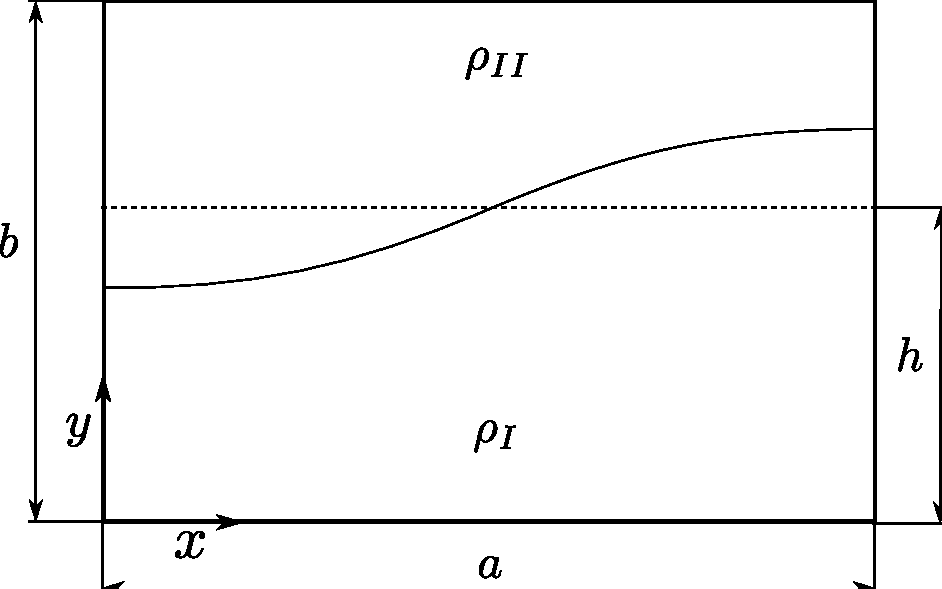
\includegraphics[width=.6\columnwidth]{images/ansari_config.pdf}
  \end{center}
  \caption{\label{fg:ansari-config} Configuration of the Non-linear sloshing in a rectangular container case. Initial condition is represented by dashed lines. Continuous line represents the position of the free-surface for a certain time.}
\end{figure}

For the different cases in this report, a 2D rectangular tank $a=1.0[m]$ width by $b=1.0[m]$ height is used. The initial height of the interface is $h=0.5[m]$ and the lateral excitation applied is $x=0.05\sin(3t)$. The simulations were performed considering the
flow as laminar and non-viscous, hence no turbulence model was used and slip boundary conditions are taken. The density ratio $\sigma=\frac{\rho{II}}{\rho{I}}$ was modified to study the density influence on the free surface evolution. A two dimensional Cartesian mesh of $450\times225$, splitted into triangles, has been used in all cases.

Reference results for this case are taken from \cite{Goni13} which uses the codes STARCCM+ and \OF to obtain numerical solutions and reports the free surface displacement on the left wall of the container. Those simulations use the same grid as presented above, but, in order to avoid numerical instabilities, the $CFL$ number was limited to $CFL_{max}=0.5$ which implies $\Delta t \approx 0.001$. In PFEM-2 simulations such restrictions do not exist, then $\Delta t$ is fixed to $0.01$, reaching $CFL_{max}\approx5$.
Figure \ref{fg:ansari-results} presents the free surface displacement reported on the left wall of the container for different density ratios. For each one of them, PFEM-2 simulations shows a good agreement with reference solutions. It is worth mentioning that the time step used is around ten times bigger than the used in \cite{Goni13}.


  \begin{figure}
  \centering
    \subfloat[]{
	  \label{fg:ansari-1}         %% Etiqueta para la primera subfigura
	  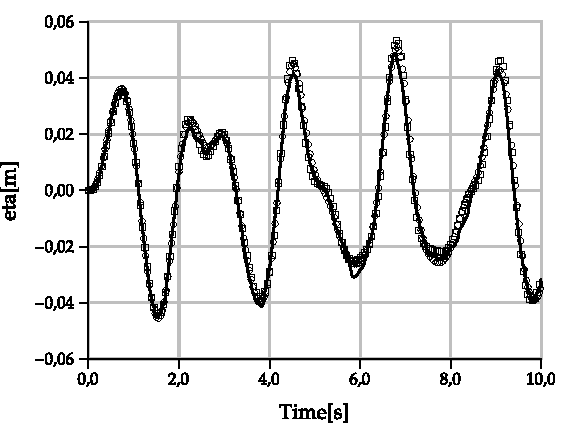
\includegraphics[width=.49\columnwidth]{images/ansari_1.pdf}
    }
    %%----segunda subfigura----
    \subfloat[]{
	  \label{fg:ansari-2}         %% Etiqueta para la segunda subfigura
	  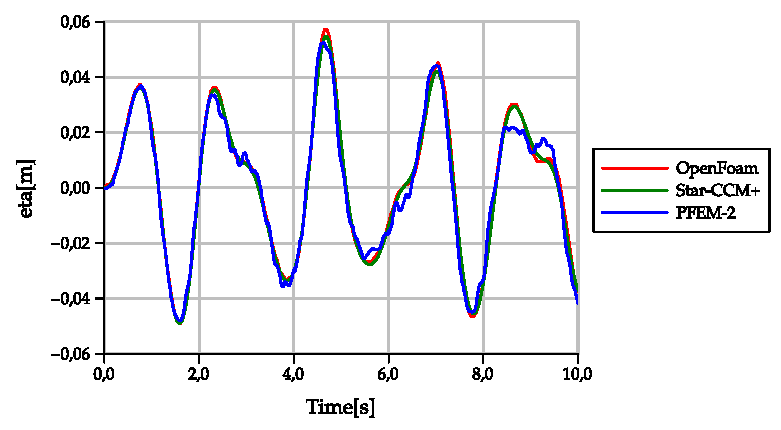
\includegraphics[width=.49\columnwidth]{images/ansari_2.pdf}
    } \\
    \subfloat[]{
	  \label{fg:ansari-3}         %% Etiqueta para la primera subfigura
	  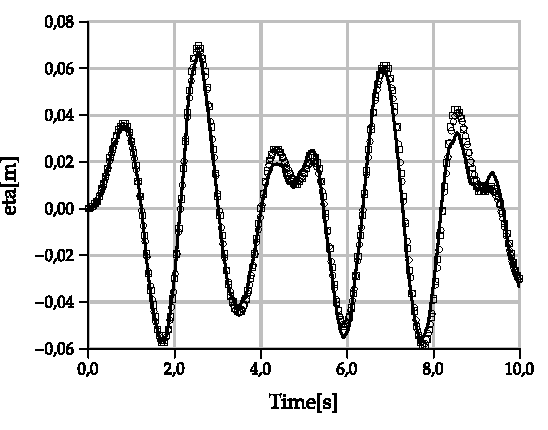
\includegraphics[width=.49\columnwidth]{images/ansari_3.pdf}
    }
    %%----segunda subfigura----
    \subfloat[]{
	  \label{fg:ansari-4}         %% Etiqueta para la segunda subfigura
	  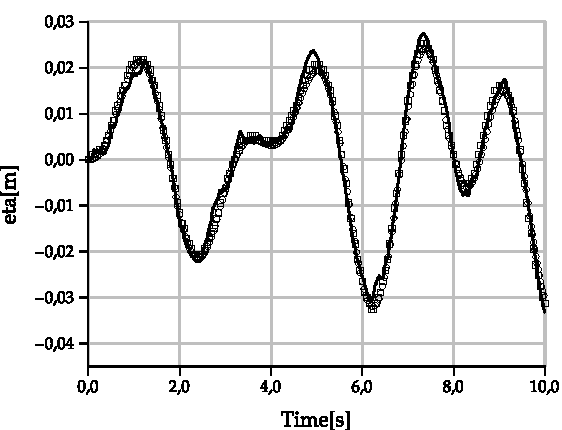
\includegraphics[width=.49\columnwidth]{images/ansari_4.pdf}
    }
   \caption{Level of height on the left wall for a two phase flow for different density ratios. Figure \ref{fg:ansari-1}: $\sigma=0.0013$, Figure \ref{fg:ansari-2}: $\sigma=0.05$, Figure \ref{fg:ansari-3}: $\sigma=0.2$ and Figure \ref{fg:ansari-4}: $\sigma=0.8$. References:\ \Circle \ STARCCM, \Square \ OpenFOAM and filled line PFEM-2.}
   \label{fg:ansari-results}                %% Etiqueta para la figura entera
\end{figure}



\subsection{Viscous standing waves}%Re=250,2500.

Computing the dissipation due to wave-breaking remains a challenging problem in the computational fluid mechanics context. In order to analyze the solution with PFEM-2 of two-phase viscous incompressible flows, the evolution of a viscous standing wave has been chosen. This is a classical problem in the scientific literature for which an approximate analytical solution is available for small amplitude perturbations\cite{Lighthill01} and it is of practical interest since it is related to the propagation of gravity waves.

The chosen standing wave configuration consists in a rectangular tank with length $L$ and a water filling height of $H = L/2$. This setup is taken from \cite{Colagrossi12}, and in the Figure \ref{fg:standing-wave-config} a sketch of this configuration is displayed. The wave length is $\lambda = L$, $k$ is the corresponding wave number (i.e. $k = 2\pi/\lambda$), $A$ is the wave amplitude and denotes the ratio $\epsilon=2A/H$.

\begin{figure}
  \begin{center}
      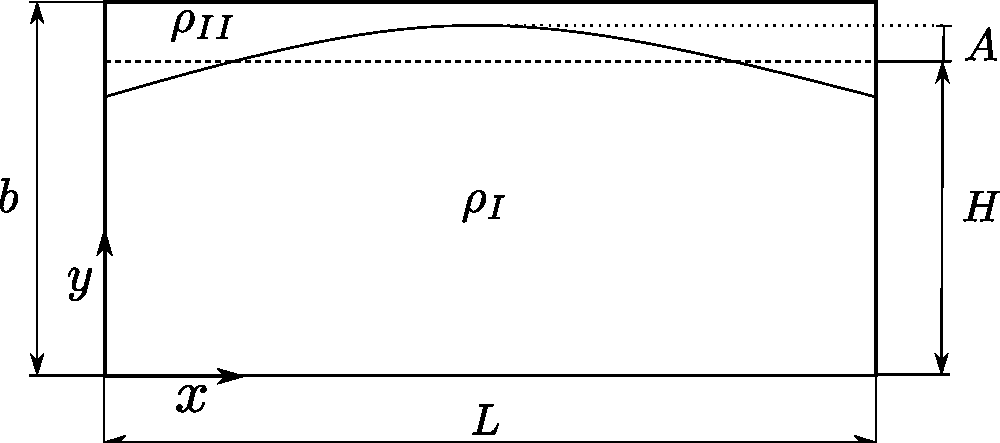
\includegraphics[width=.9\columnwidth]{images/standing_wave.pdf}
  \end{center}
  \caption{\label{fg:standing-wave-config} Configuration scheme of standing wave case. Initial condition is represented by dotted lines. In continuous line is presented an intermediate state where the maximum amplitude $A$ is reached.}
\end{figure}

If the fluid is viscous, the dissipation due to the solid boundary layers is neglected, small-amplitude waves (i.e small $\epsilon$) and small wave steepness (i.e $2A/\lambda \ll 0.1$) are used; an approximate analytical solution of the standing wave evolution can be obtained through the linearization of Navier-Stokes equations for traveling waves:
\begin{align}
 \varphi(x,y,t) & = \varphi_0(x,y)\cos(\omega t) \\
 \varphi_0(x,y) & =-\epsilon\frac{Hg}{2\omega}\frac{\cosh\left[k(y+H)\right]}{\cosh(kH)}\cos(kx)
\end{align}

where the circular frequency $\omega$ is given by the dispersion relation of gravity waves, that is, $\omega^2 = g k \tanh(kH)$ where $g$ is the acceleration of gravity. At time $t = 0$ the free surface is horizontal while the initial fluid velocity is given by $\varphi_0$.

It can be demonstrated that the approximate solution is well posed only for $Re\gg1$ and for $Re^{-1}\ll k \ll Re^{2/3}$, where $Re=H\sqrt{gH}/\nu$ is the Reynolds number for this problem. From that solution, it is possible to obtain the formula that gives the approximate decay of the kinetic energy\cite{Lighthill01}:

\begin{equation}
 \varepsilon_K(t) = \epsilon^2g\frac{\lambda H^2}{32}e^{-4\nu k^2t}\left[1+\cos(2\omega t)\right]
 \label{kin-eq}
\end{equation}

The kinetic attenuation is governed by the coefficient of the exponential $\beta_l = 4\nu k^2$, which depends on the wave number and on the kinematic viscosity $\nu = \mu/\rho_{I}$. Lately work\cite{Antuono13} has demonstrated that generally, the Equation \ref{kin-eq} overestimates the dissipations, especially when the Reynolds number is not very large. Then an improved damping rate is proposed in that paper $\beta = 4\nu k^2 -  2\sqrt{2}k^{11/4}Re^{-3/2}+O(Re^{-2})$, which is next used for comparisons.

To accomplish the linear solution hypothesis, the PFEM-2 simulations have been implemented by using a free-slip condition for the velocity and a Neumann condition for the pressure along each boundary of the tank. Also, the parameters $L=2$, $A=0.05$ and $g=1$ have been selected.

Several Reynolds number ($Re=25,50,250,2500$) have been selected to compare with the approximate analytic dissipation. Problems were solved into a grid with $H/\Delta x=100$ and varying $\Delta t$ in order to solve using a Fourier number $Fo=\frac{\nu\Delta t}{\Delta x^2}$ with a local maximum of $Fo_{max}\approx10-50$. Figure \ref{fg:sw-energy} shows the comparison between the expected dissipation (which includes the improving damping rate) and numerical results with PFEM-2. Large Fourier numbers were used in order to reduce the computation times required to complete the simulations and to show the accuracy of the method working not only with large CFL numbers, even with large diffusion rate.

  \begin{figure}
  \centering
    \subfloat[]{
	  \label{fg:sw-energy-25}
	  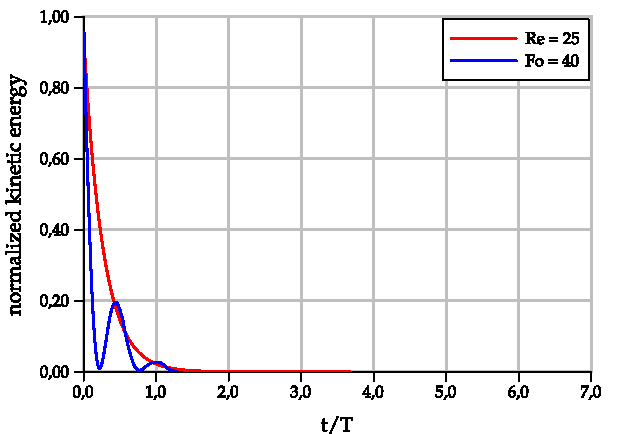
\includegraphics[width=.72\columnwidth]{images/sw_25.pdf}
    } \\
    \subfloat[]{
	  \label{fg:sw-energy-50}
	  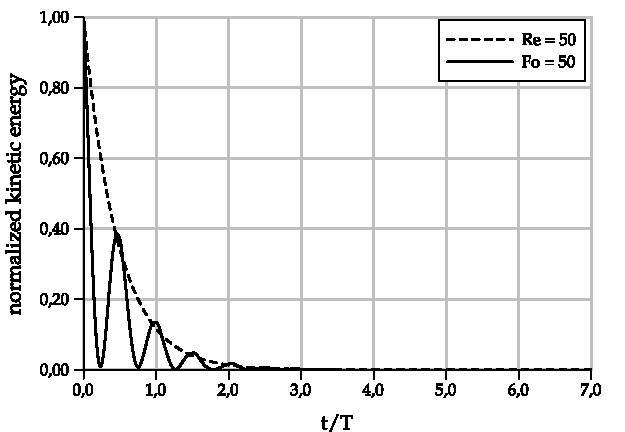
\includegraphics[width=.72\columnwidth]{images/sw_50.pdf}
    } \\
    \subfloat[]{
	  \label{fg:sw-energy-250}
	  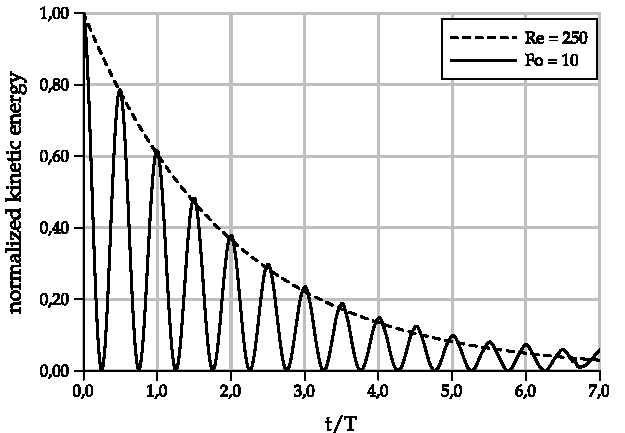
\includegraphics[width=.72\columnwidth]{images/sw_250.pdf}
    } \\
    \subfloat[]{
	  \label{fg:sw-energy-2500}
	  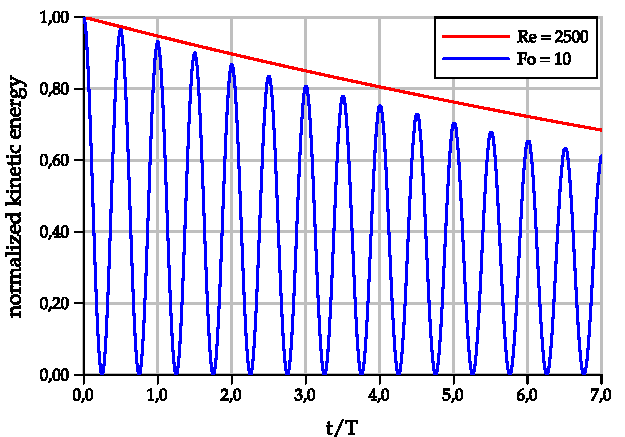
\includegraphics[width=.72\columnwidth]{images/sw_2500.pdf}
    }
   \caption{Kinetic Energy decay for standing wave problem with different Reynolds numbers. Red lines are approximate analytical solutions for total energy and blue lines are numerical solutions with PFEM-2. Reynolds numbers analyzed: $Re=25,50,250,2500$ in Figures \ref{fg:sw-energy-25},\ref{fg:sw-energy-50},\ref{fg:sw-energy-250},\ref{fg:sw-energy-2500} respectively. Legend in each figure indicates the maximum Fourier number used in each numerical simulation.}
   \label{fg:sw-energy}
\end{figure}

\subsection{Rayleigh-Taylor Instability}

This problem consists on the evolution of two layers of fluids initially at rest in the gravity field. The density of the fluid placed at the top is larger than the one placed at the bottom. Due to a little disturbance in the contact surface the more dense fluid goes down and the less dense fluid does the opposite. During the evolution of the problem a mixture is created, which is lately segregated. The final state reaches an stable equilibrium with the more dense fluid at the bottom layer and the less dense fluid at the top layer. The growth and evolution of the instability has been investigated among others by Tryggvason\cite{Tryggvason88} for inviscid incompressible flows, and by Guermond \& Quartapelle\cite{Guermond00} for viscous flows.

The starting point is the problem documented by Guermond. The computational domain is $[-d/2,-2d]\times[d/2,2d]$ and the initial position of the perturbed interface is $\eta(x) = 0.1d \cos(2\pi x/d)$. The density ratio is $3$, which corresponds to an Atwood
number of $0.5$ according to Tryggvason's definition $At = (\rho_{max}-\rho_{min})/(\rho_{max}+\rho_{min})$. Other physical parameters are selected to obtain a Reynolds number $Re=\rho_{min}d^{\frac{3}{2}}g^{\frac{1}{2}}/\mu=1000$. The computational domain is discretized into $80000$ structured triangles ($\Delta x=0.01$) setting slip boundary conditions on each wall. Time step selected is $\Delta t=0.01[s]$, which allows to reach $CFL_{max} \approx 8$. Between five and eight particles per element are used and two pressure corrections are required.

To compare with reference results, the time is made dimensionless by using $\widetilde{t} = t\sqrt{g\ At}$. Results on the vertical position of the tip of the falling and rising fluid (spike and bubble, respectively) are shown in Figure \ref{fg:rayleigh-rf}. It can be observed that current solution is in good agreement with the reference results.

\begin{figure}
  \begin{center}
      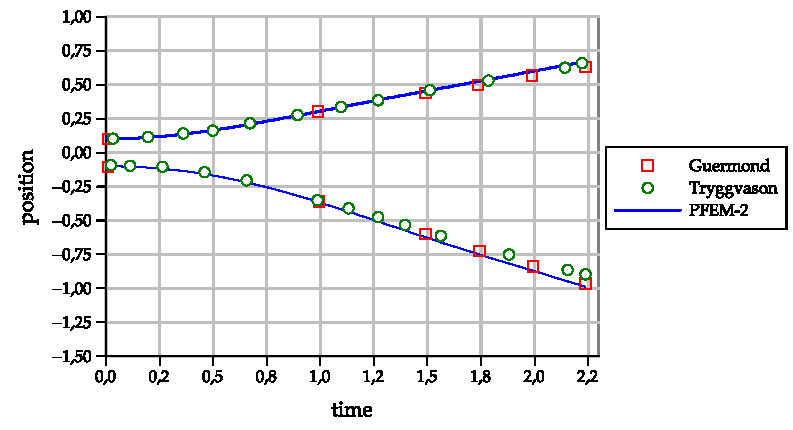
\includegraphics[width=\columnwidth]{images/rayleigh_1.pdf}
  \end{center}
  \caption{\label{fg:rayleigh-rf} Position of rising and falling bubbles versus time. Case with $Re=1000$.}
\end{figure}

On the other hand, the evolution of the instability is shown in Figure \ref{fg:rayleigh-screenshots} at dimensionless times $\widetilde{t}=0, 1, 1.5, 2$. Around $\widetilde{t}=1.5$ the heavy fluid begins to roll up into two counter-rotating vortices. Later, around $\widetilde{t} = 2$, these two vortices become unstable and a pair of secondary vortices appear at the tails of the roll-ups. These shapes of the fluid interface obtained with PFEM-2 are similar to the ones shown as reference results, see \cite{Guermond00}.


\begin{figure}
  \begin{center}
      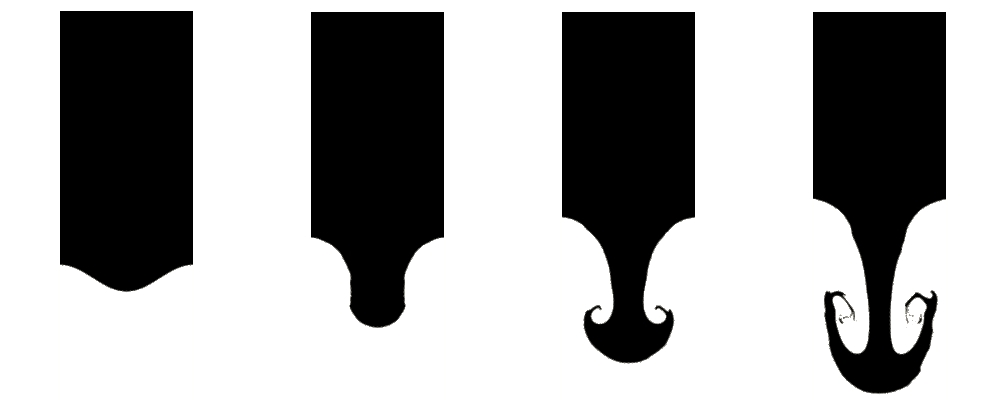
\includegraphics[width=\columnwidth]{images/rayleigh_2_better.jpg}
  \end{center}
  \caption{\label{fg:rayleigh-screenshots} Rayleigh-Taylor instability evolution. Case with $Re=1000$. From left to right $\widetilde{t} =0.0$, $1.0$, $1.5$, $2.0$.}
\end{figure}

\subsubsection{Extending the time step}

In order to make emphasis in the capability of the method to manage large time-steps, the current case is also simulated with a large range of $\Delta t$ using the in-house implementation of PFEM and comparing with results obtained by the widely knows \OF suite. The problem setup and domain discretization is the same as presented above and the PFEM settings are not modified.


Figure \ref{fg:rayleigh-comparison-dts} presents the comparison of the solutions with PFEM and \OF at a particular time ($\widehat{t}=2.25$) using several fixed time-steps (with the largest time-step a $CFL_{max}=15$ is reached). From captures, it can be shown that PFEM keeps approximately the same solution with each time-step, but interFoam can not solve with any accuracy using $\Delta t>0.001$ because the evolution of the mushroom-like interface differs form the reference results and this mistake is increased with large time-steps. Moreover, each simulation of interFoam diverges when $CFL_{mean}>0.5$ is reached (this happens at different times, depending on selected time-step).

\begin{figure}
  \begin{center}

      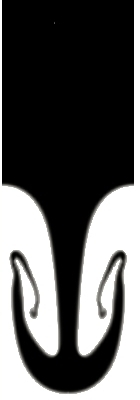
\includegraphics[width=.24\columnwidth]{images/rayleigh_foam_dts_A.jpg}
      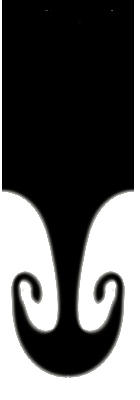
\includegraphics[width=.24\columnwidth]{images/rayleigh_foam_dts_B.jpg}
      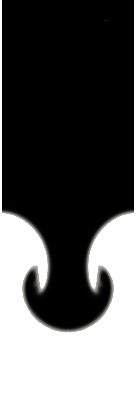
\includegraphics[width=.24\columnwidth]{images/rayleigh_foam_dts_C.jpg}
      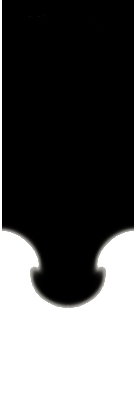
\includegraphics[width=.24\columnwidth]{images/rayleigh_foam_dts_D.jpg}

      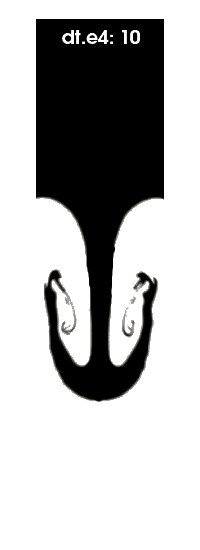
\includegraphics[width=.24\columnwidth]{images/rayleigh_pfem_dts_A.jpg}
      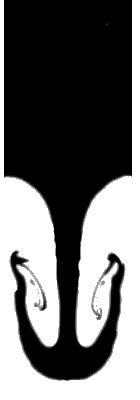
\includegraphics[width=.24\columnwidth]{images/rayleigh_pfem_dts_B.jpg}
      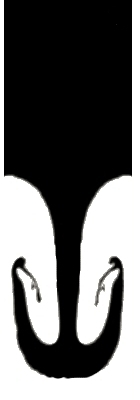
\includegraphics[width=.24\columnwidth]{images/rayleigh_pfem_dts_C.jpg}
      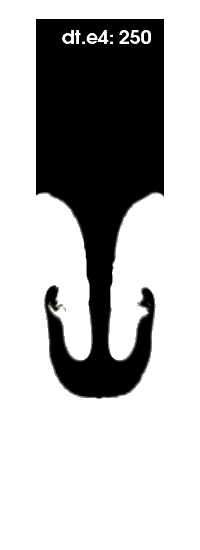
\includegraphics[width=.24\columnwidth]{images/rayleigh_pfem_dts_D.jpg}

  \end{center}
  \caption{\label{fg:rayleigh-comparison-dts} Rayleigh-Taylor instability capture for $\widetilde{t}=2.25$. Bottom: PFEM simulations, top: VoF+MULES simulation (InterFoam solver - OpenFoam suite). From left to right $\Delta t =0.001[s]$, $0.0025[s]$, $0.01[s]$, $0.025[s]$.}
\end{figure}

Another relevant feature to take into account is that the CPU times to solve a unique time-step is almost equal using both algorithms.
% Table \ref{tb:times-rt} shows a resume of the CPU Times requires to complete $1[s]$ of real time in the current case.
In current case,  the only reasonable solution of \OF among the ones presented above is that with $\Delta t=0.001$. For that simulation, using a processor Intel i5-3230M CPU @ 2.60GHz with a 8Gb RAM in one processor, interFoam requires $1121[s]$ to reach $1[s]$ of simulation time. On the other hand, to reach the same simulation time using the same computer, solutions with PFEM-2 requires $1011[s]$, $288[s]$ and $123[s]$ with $\Delta t=0.0025[s]$, $0.01[s]$ and $0.025[s]$ respectively.




\subsubsection{Three-dimensional simulation}

In this section, the extension of the two dimensional problem to three dimensions is presented. The third dimension is generated as a surface of revolution from the previous 2d geometry, conforming a cylindrical volume in 3d of radius $R=0.5$. This allows to keep the same problem configuration, it is slip boundary condition on the wall, $At=0.5$, and initial perturbation of the surface $\eta(r) = 0.1d \cos(2\pi r/d)$, with $0<r<R$.

Computational domain is discretized with a mesh size of $\Delta x=0.03[m]$ conforming a non-structured mesh with around $1.2$ millon of tetrahedral elements. An average of eight millon of particles are used during the simulation that move across the light-phase and heavy-phase domains. Simulation was carried out with a $\Delta t=0.025$ which allows to reach peaks of $CFL_{max}=15$. In the Figure \ref{fg:rayleigh-3d} can be shown the evolution of the heavy-phase. It must be noticed that the simulation is extended long time up to reach the stable condition with heavy-phase at bottom and at rest, which is approximately $30[s]$ of simulation time. To complete the entire simulation, the implementation requires around three hours of CPU time running in an AMD Opteron 6376 @ 2.3GHz with a 64Gb RAM using 16 processors.

As a additional result, it is important to underline that during the simulation the global mass conservation has been checked.

 However, the spirit of this section is to show the stability of the 3D simulation, keeping a realistic progress. A way to prove the goodness of the solution is that, during the simulation, the initial mass quantity is preserved. More detailed analysis about the accuracy of 3d simulations will be presented in Section \ref{sec:ETSIN-3d}.

\begin{figure}
  \begin{center}
    \subfloat[]{
	  \label{fg:RT-3d-a}
	  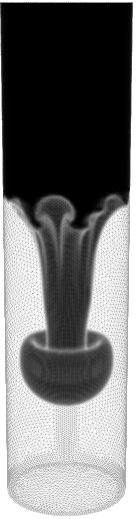
\includegraphics[width=.18\columnwidth]{images/RT_3d/RT3d_a.jpg}
    }
    \subfloat[]{
	  \label{fg:RT-3d-b}
	  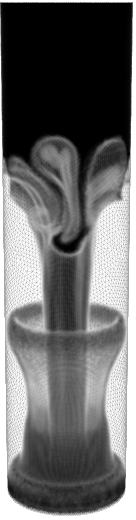
\includegraphics[width=.18\columnwidth]{images/RT_3d/RT3d_b.jpg}
    }
    \subfloat[]{
	  \label{fg:RT-3d-c}
	  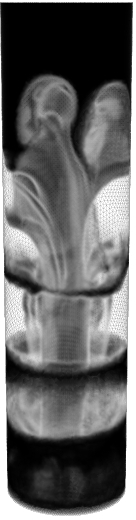
\includegraphics[width=.18\columnwidth]{images/RT_3d/RT3d_c.jpg}
    }
%     \subfloat[]{
% 	  \label{fg:RT-3d-d}
% 	  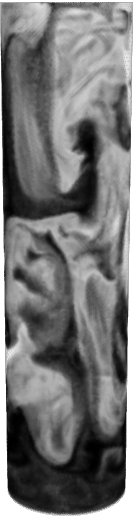
\includegraphics[width=.15\columnwidth]{images/RT_3d/RT3d_d.jpg}
%     }
    \subfloat[]{
	  \label{fg:RT-3d-e}
	  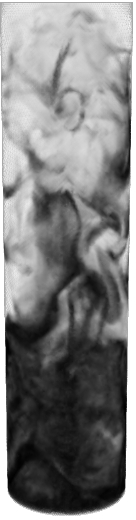
\includegraphics[width=.18\columnwidth]{images/RT_3d/RT3d_e.jpg}
    }
    \subfloat[]{
	  \label{fg:RT-3d-g}
	  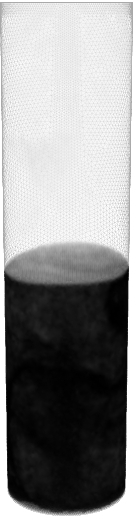
\includegraphics[width=.18\columnwidth]{images/RT_3d/RT3d_g.jpg}
    }
  \end{center}
  \caption{\label{fg:rayleigh-3d} Snapshots of the heavy-phase in the Rayleigh-Taylor instability solved in three-dimensions with PFEM-2. %From left to right $\widetilde{t} =2[s]$, $3.3[s]$, $4.4[s]$, $6.6[s]$, $8,8[s]$, and $27.5[s]$.}
  From left to right $\widetilde{t} =2[s]$, $3.3[s]$, $4.4[s]$, $8,8[s]$, and $27.5[s]$.}
\end{figure}

\subsection{Dam-break problem}%ETSIN experimental tests

The objectives of this section are to compare experimental measurements on dam-break flow over a dry horizontal bed with the numerical approximation carried out with the PFEM-2 algorithm. The extensive set of experimental data is extracted from \cite{Lobovsky13}, where the dynamics of the dam break wave impacting a vertical wall downstream the dam, with emphasis on the pressure loads and surface evolution after the dam burst, are presented.

Computational configuration of the tank used in experimental cases is presented in Figure \ref{fg:dambreak-config}, where the locations of water level measuring points and pressure sensors are shown. In this report only the case with $H=300[mm]$ is analyzed. Two-phase non-viscous flow simulation is carried on, with $\rho_{water}=1000[kg/m^3]$, $\rho_{air}=1[kg/m^3]$ and gravity force $\mathbf{g}=-10\ \hat{j} [m/s^2]$. The 2D computational grid used has $322\times120$ nodes, conforming a mesh with around $80000$ triangles. Boundary conditions are slip on all walls, and $\Delta t$ is fixed to $0.1$, which allows to reach $CFL_{max}\approx20$ when free surface impacts the downstream wall.

\begin{figure}
  \begin{center}
      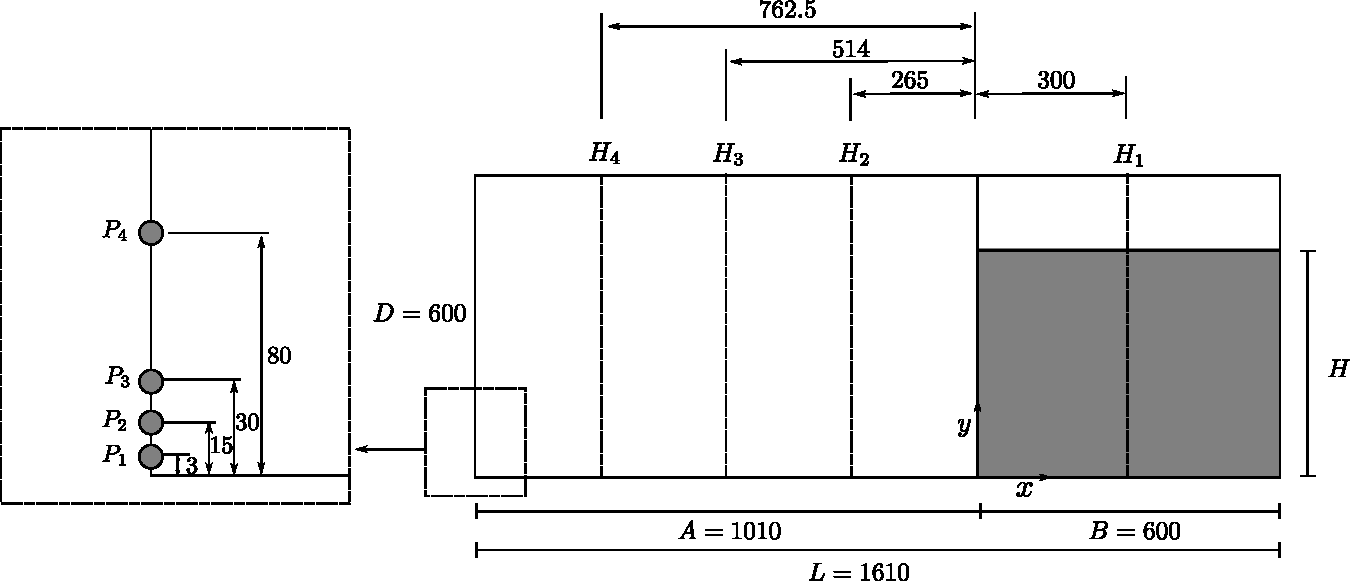
\includegraphics[width=\columnwidth]{images/dam_break_config.pdf}
  \end{center}
  \caption{\label{fg:dambreak-config} Configuration scheme of the dam-break case. $H_1$, $H_2$, $H_3$, $H_4$ present the locations of water level measuring positions. Also, $P_1$, $P_2$, $P_3$, $P_4$ show the locations of pressure sensors at the impact wall downstream the dam. Grey zone represents the initial condition. Dimensions in millimeters.}
\end{figure}

Figure \ref{fg:dambreak-h} shows the comparison between experimental and numerical results for each water-level measurement. A good agreement can be observed, moreover taken into account the capture of the back wave and splashing start events.
  \begin{figure}
  \centering
    \subfloat[]{
	  \label{fg:dambreak-h1}         %% Etiqueta para la primera subfigura
	  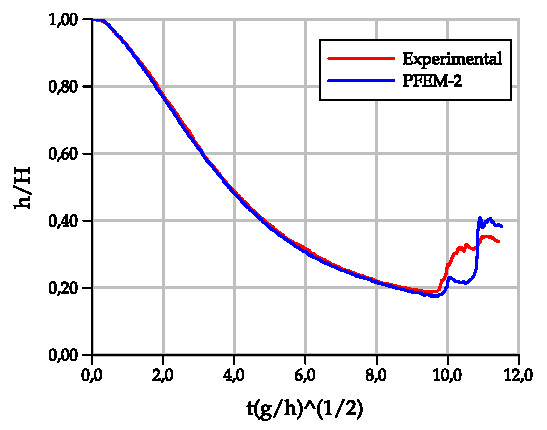
\includegraphics[width=.49\columnwidth]{images/dambreak_h1.pdf}
    }
    %%----segunda subfigura----
    \subfloat[]{
	  \label{fg:dambreak-h2}         %% Etiqueta para la segunda subfigura
	  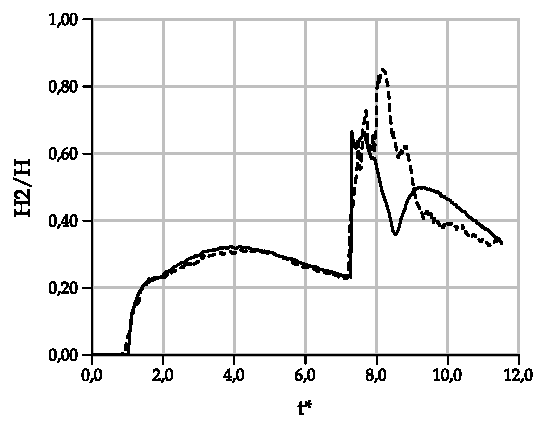
\includegraphics[width=.49\columnwidth]{images/dambreak_h2.pdf}
    } \\
    \subfloat[]{
	  \label{fg:dambreak-h3}         %% Etiqueta para la primera subfigura
	  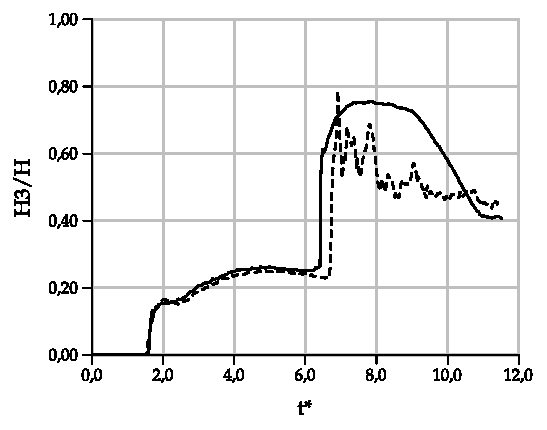
\includegraphics[width=.49\columnwidth]{images/dambreak_h3.pdf}
    }
    %%----segunda subfigura----
    \subfloat[]{
	  \label{fg:dambreak-h4}         %% Etiqueta para la segunda subfigura
	  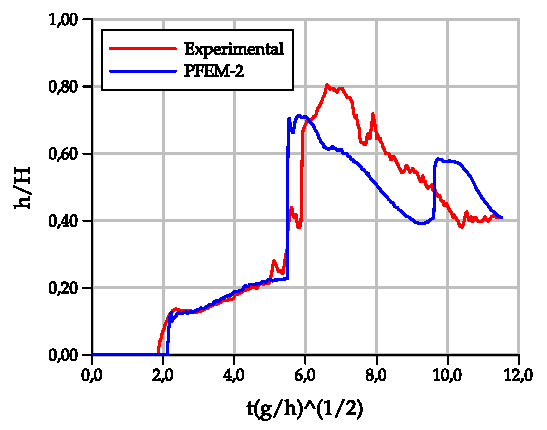
\includegraphics[width=.49\columnwidth]{images/dambreak_h4.pdf}
    }
   \caption{Water level elevations at locations $H_1$, $H_2$, $H_3$ and $H_4$ for tests with $H=300[mm]$ initial filling height compared to data from literature experimental results\cite{Lobovsky13} (dashed lines) and numerical results with PFEM-2 (filled lines). Time normalization is $t^*=t(g/h)^{1/2}$.}
   \label{fg:dambreak-h}                %% Etiqueta para la figura entera
\end{figure}

The impact pressure was measured with four sensors at the vertical wall at the end of the downstream flume, as described in Figure \ref{fg:dambreak-config}. The statistical analysis of the pressure peaks, rise times and the occurrence time, i.e. the time between
the opening of the dam gate and the occurrence of the impact, are presented in Figure \ref{fg:dambreak-p}. The shown pressure $P$ is non-dimensionalized with regards to the hydrostatic pressure at the bottom of the reservoir.

In the reference work, the analysis is focused on peaks events. It can be noticed that the highest peak is recorded by sensor number 1 which is the sensor receiving the full impact, whilst the pressure of the other sensors is given by the run up of the flow. It can also be observed that sensor number 4, i.e. the sensor located at the highest position, does not show a pure impact event, see Figure \ref{fg:dambreak-p4}, and actually the maximum for this sensor is obtained later in time, when the water falls back after running along the wall. Numerical solution behavior follows the mentioned conclusions, but the pressure values are not between the statistical limits of experimental data. Also, a discrepancy can be observed with the peaks arrival times for sensors $1$ to $3$. This difference can be assigned to the numerical simplification which does not model the gate movement. However, pressure magnitude of the peaks is well predicted giving confidence to PFEM-2 calculations.

  \begin{figure}
  \centering
    \subfloat[]{
	  \label{fg:dambreak-p1}         %% Etiqueta para la primera subfigura
	  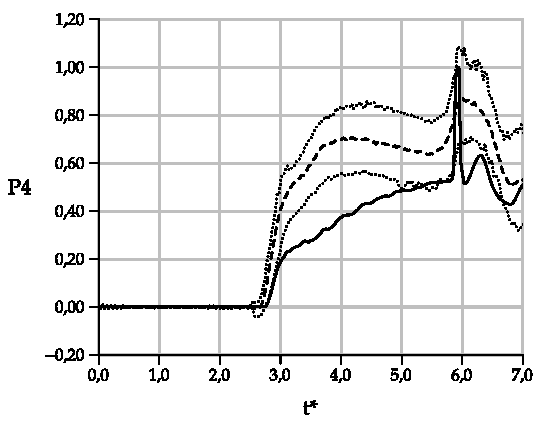
\includegraphics[width=.48\columnwidth]{images/dambreak_p4.pdf}
    }
    %%----segunda subfigura----
    \subfloat[]{
	  \label{fg:dambreak-p2}         %% Etiqueta para la segunda subfigura
	  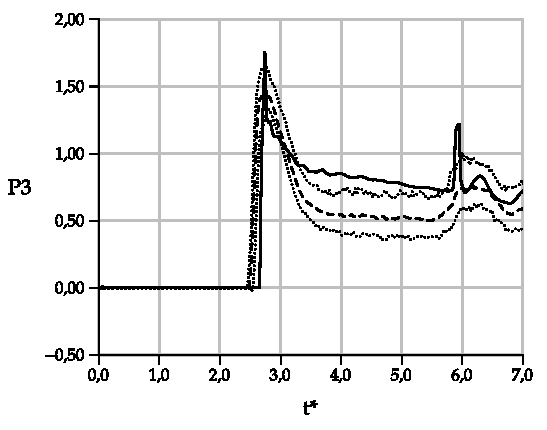
\includegraphics[width=.48\columnwidth]{images/dambreak_p3.pdf}
    } \\
    \subfloat[]{
	  \label{fg:dambreak-p3}         %% Etiqueta para la primera subfigura
	  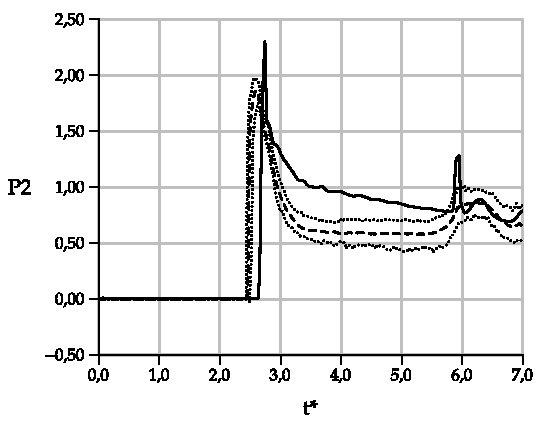
\includegraphics[width=.48\columnwidth]{images/dambreak_p2.pdf}
    }
    %%----segunda subfigura----
    \subfloat[]{
	  \label{fg:dambreak-p4}         %% Etiqueta para la segunda subfigura
	  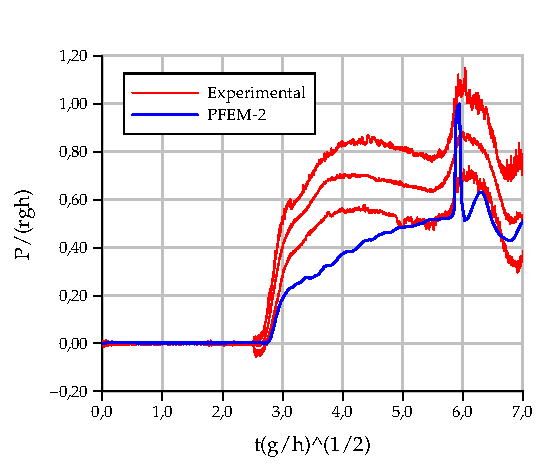
\includegraphics[width=.48\columnwidth]{images/dambreak_p1.pdf}
    }
   \caption{Pressure time histories comparison between experimental results\cite{Lobovsky13} (discontinuous lines) and numerical results with PFEM-2 (filled lines). Locations $P_1$, $P_2$, $P_3$, $P_4$ are presented in Figures \ref{fg:dambreak-p1},\ref{fg:dambreak-p2},\ref{fg:dambreak-p3},\ref{fg:dambreak-p4} respectively. Experimental results shows the median (dashed lines) and percentiles $2.5$ and $97.5$ (dotted lines).}
   \label{fg:dambreak-p}                %% Etiqueta para la figura entera
\end{figure}

Finally, the Figure \ref{fg:dambreak-screenshots} presents snapshots for the evolution of the free-surface simulation. Initial condition is shown in Figure \ref{fg:dambreak-1}. Pressure peaks are related with the impact event observed in Figure \ref{fg:dambreak-3}, which generates the back wave propagation that is displayed in remain figures.
\begin{figure}
  \centering
    \subfloat[]{
	  \label{fg:dambreak-1}
	  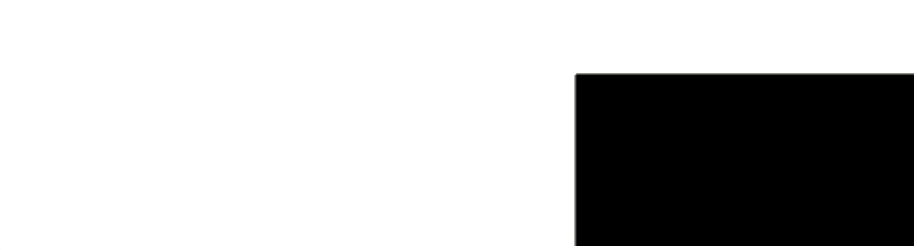
\includegraphics[width=.48\columnwidth]{images/dambreak_pfem_1_w.jpg}
    }
    %%----segunda subfigura----
    \subfloat[]{
	  \label{fg:dambreak-2}
	  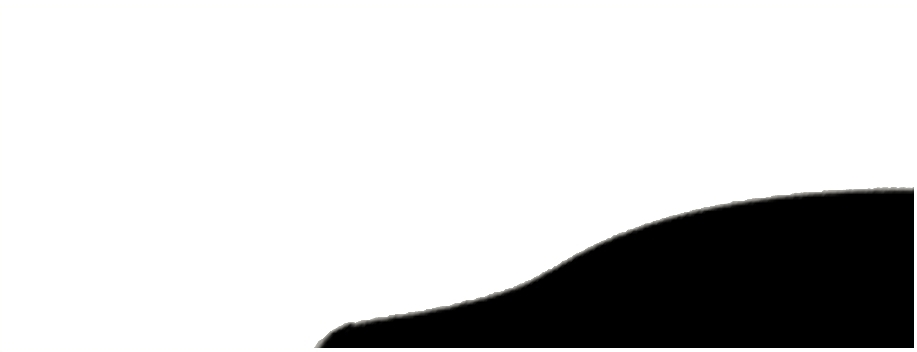
\includegraphics[width=.48\columnwidth]{images/dambreak_pfem_2_w.jpg}
    } \\
    \subfloat[]{
	  \label{fg:dambreak-3}
	  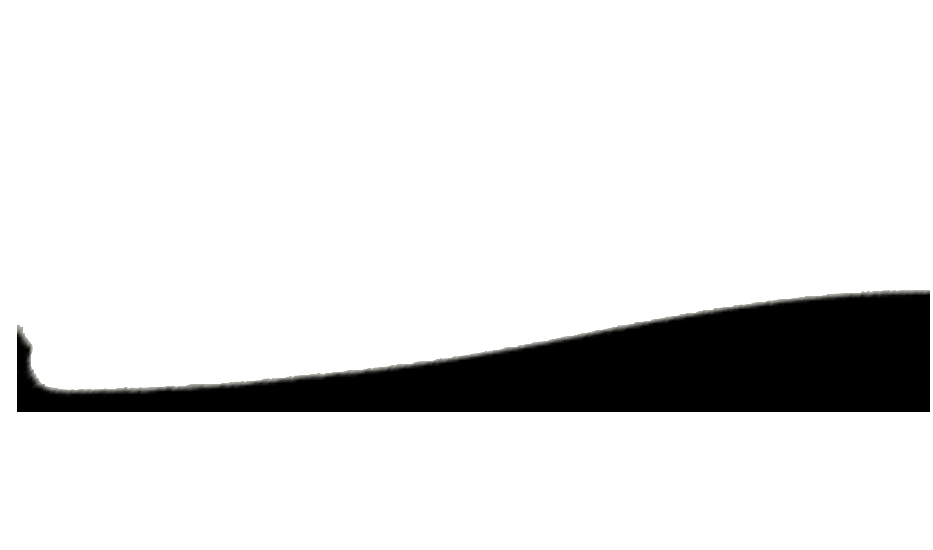
\includegraphics[width=.48\columnwidth]{images/dambreak_pfem_3_w.jpg}
    }
    %%----segunda subfigura----
    \subfloat[]{
	  \label{fg:dambreak-4}
	  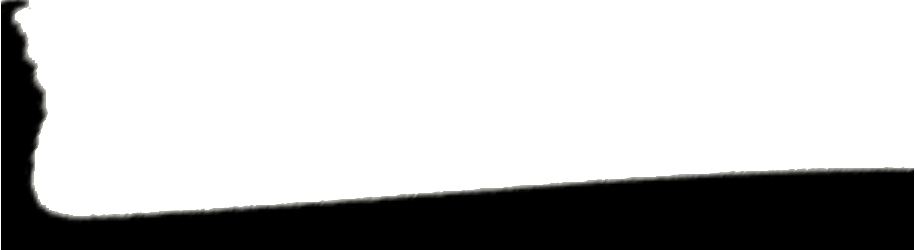
\includegraphics[width=.48\columnwidth]{images/dambreak_pfem_4_w.jpg}
    }\\
        \subfloat[]{
	  \label{fg:dambreak-5}
	  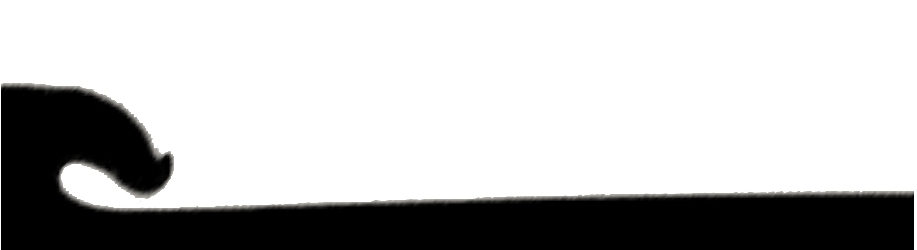
\includegraphics[width=.48\columnwidth]{images/dambreak_pfem_5_w.jpg}
    }
    %%----segunda subfigura----
    \subfloat[]{
	  \label{fg:dambreak-6}
	  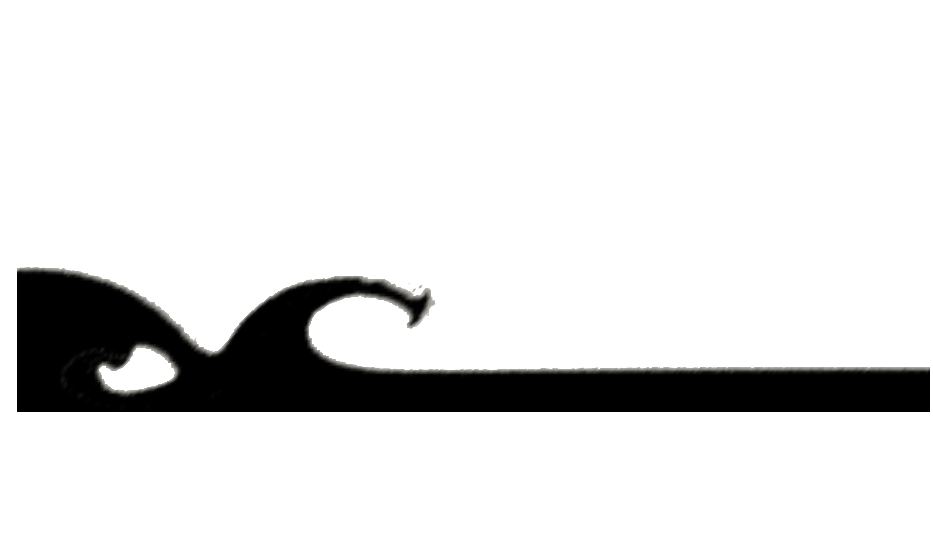
\includegraphics[width=.48\columnwidth]{images/dambreak_pfem_6_w.jpg}
    } \\
    \subfloat[]{
	  \label{fg:dambreak-7}
	  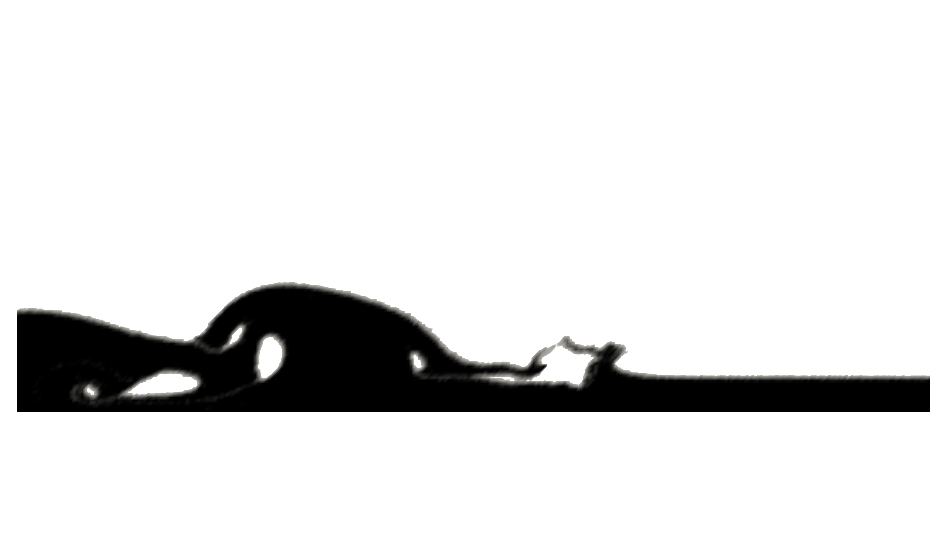
\includegraphics[width=.48\columnwidth]{images/dambreak_pfem_7_w.jpg}
    }
    %%----segunda subfigura----
    \subfloat[]{
	  \label{fg:dambreak-8}
	  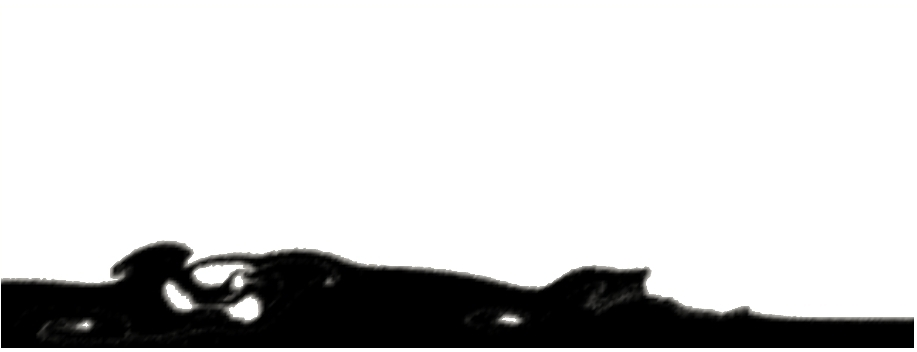
\includegraphics[width=.48\columnwidth]{images/dambreak_pfem_8_w.jpg}
    }
   \caption{Snapshots of the dam-break at times $t=0$, $0.25$, $0.5$, $0.75$, $1$, $1.25$, $1.5$, $1.75[s]$, in Figures \ref{fg:dambreak-1} to \ref{fg:dambreak-8} respectly.}
   \label{fg:dambreak-screenshots}
\end{figure}
\clearpage

\subsubsection{Three-dimensional Simulation}\label{sec:ETSIN-3d}

Despite being a problem that can be accurately simulated in 2D, the same example was run in 3D to test the ability of the PFEM-2 solver to deal with larger geometries and 3D problems. The 3D mesh, which adds a third dimension of a thickness of $0.15[m]$ with slip walls, has six million of elements with an average $h=0.07$, demanding more than $25$ million particles for the fixed mesh approximation that move across the air and water domains. The same physical and numerical parameters of the 2D simulation were used. Sensors are placed in the same position of the left wall and in the middle position of the third dimension.

In this example, the time step used, the element sizes and the velocity of the fluid lead to a simulation with some time-steps having a Courant number larger than 12, mainly at the moment of wave impacts with walls. This shows again the capability of the method to manage 3D geometries with large time-steps. In Figure \ref{fg:dambreak-p-3d} the pressure history for each sensor is presented, showing similar appearance with the two dimensional simulation.

  \begin{figure}
  \centering
    \subfloat[]{
	  \label{fg:dambreak-p1-3d}         %% Etiqueta para la primera subfigura
	  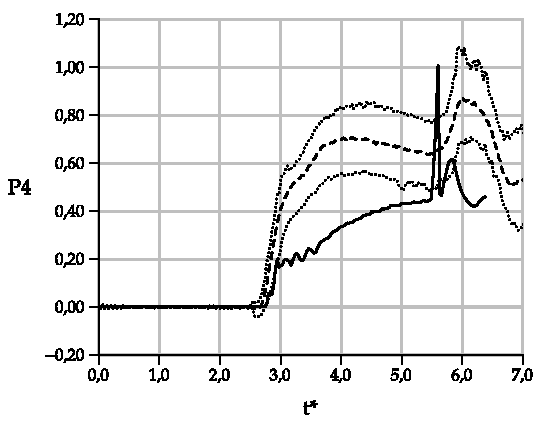
\includegraphics[width=.48\columnwidth]{images/dambreak_p4_3d.pdf}
    }
    %%----segunda subfigura----
    \subfloat[]{
	  \label{fg:dambreak-p2-3d}         %% Etiqueta para la segunda subfigura
	  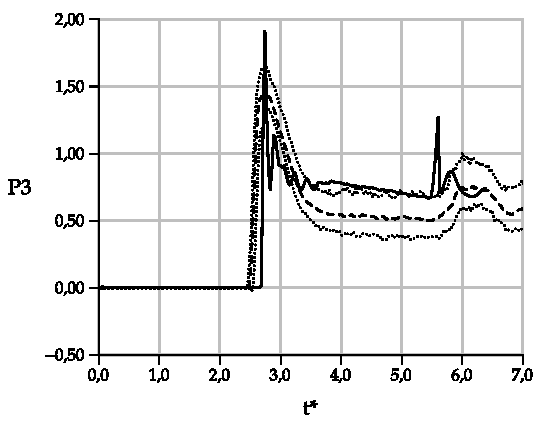
\includegraphics[width=.48\columnwidth]{images/dambreak_p3_3d.pdf}
    } \\
    \subfloat[]{
	  \label{fg:dambreak-p3-3d}         %% Etiqueta para la primera subfigura
	  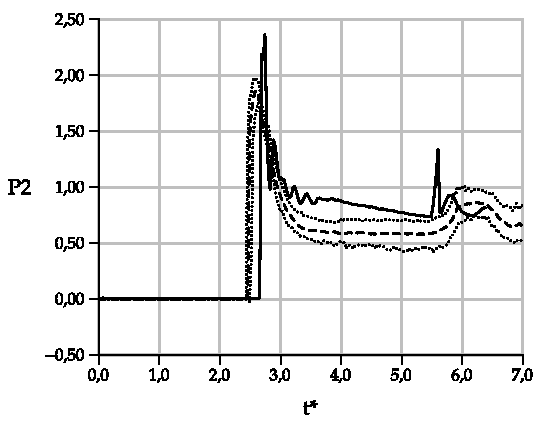
\includegraphics[width=.48\columnwidth]{images/dambreak_p2_3d.pdf}
    }
    %%----segunda subfigura----
    \subfloat[]{
	  \label{fg:dambreak-p4-3d}         %% Etiqueta para la segunda subfigura
	  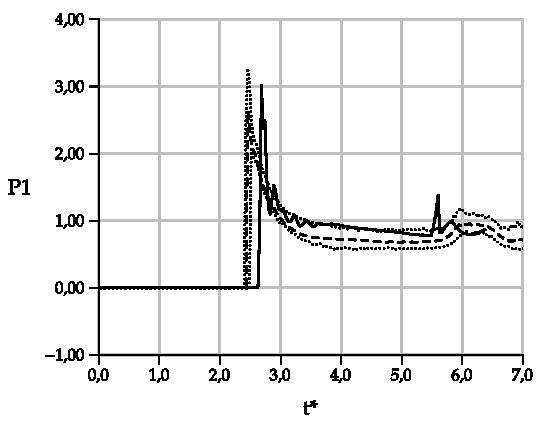
\includegraphics[width=.48\columnwidth]{images/dambreak_p1_3d.pdf}
    }
   \caption{Pressure time histories comparison between experimental results\cite{Lobovsky13} (discontinuous lines) and numerical results with PFEM-2 in three dimensions (filled lines). Locations $P_1$, $P_2$, $P_3$, $P_4$ are presented in Figures \ref{fg:dambreak-p1-3d},\ref{fg:dambreak-p2-3d},\ref{fg:dambreak-p3-3d},\ref{fg:dambreak-p4-3d} respectively. Experimental results shows the median (dashed lines) and percentiles $2.5$ and $97.5$ (dotted lines).}
   \label{fg:dambreak-p-3d}                %% Etiqueta para la figura entera
\end{figure}



\section{Conclusion}

The second generation of the Particle Finite Element Method (PFEM-2) is a novel strategy which uses a spatial discretization based on a background mesh and a cloud of particles. The dynamics equations are solved in a Lagrangian frame, where the implicit nonlinearities of the equation are solved using the {X-IVAS} strategy. That explicit temporal integration for convective terms allows to use large time-steps, then it provides a very efficient way concerning to computing times.

In the current work, a general formulation to solve free-surface flows with pressure gradient discontinuities was presented and exhaustively tested. That algorithm, which is based on a continuous enriched space for pressure, has shown good accuracy solving a wide range of multiphase problems and keeping the advantage of the possibility of using large time-steps. Several cases with a large variety of Froude numbers, density ratios and dominant dissipative cases have been analyzed, whose results were compared with other reference softwares, semi-analytical expressions and also experimental data. In each of them, PFEM-2 has proven being accurately competitive and computationally efficient. Regarding to CPU times, they can be decreased without accuracy lost if the condensing strategy for enriched pressure degrees of freedom is used. That approach loss the generality of the formulation for any range of application, but reduces the computational cost enforcing the asseveration that, to our knowledge, nowadays PFEM-2 is the faster algorithm for solving multiphase flows.

% use section* for acknowledgement
\section*{Acknowledgment}
The research leading to these results has received funding from the ARCOIRIS EU grant.
\bibliographystyle{plain}
\bibliography{mybib}


\end{document}


